\documentclass[aspectratio=169]{beamer}

\usetheme{default}
\usepackage[utf8]{inputenc}
\usepackage[brazil]{babel}
\usepackage{tikz}
\usepackage{tabularx}
\usetikzlibrary{positioning,shapes.geometric,arrows.meta}
\usepackage{amsmath}
\usepackage{booktabs}
\usepackage{multirow}
\usepackage{graphicx}
\usepackage{hyperref}
\usepackage{amssymb}
\usepackage{colortbl}

\setbeamertemplate{footline}[frame number]
\setbeamertemplate{frametitle}[default][center]

\mode<presentation>{
\usetheme{Dresden}
\usecolortheme{seagull}
}

\setbeamertemplate{headline}{}

\definecolor{peeblue}{RGB}{1,123,165}
\definecolor{darkblue}{RGB}{0,65,115}
\definecolor{lightgray}{RGB}{240,240,240}
\definecolor{goldencolor}{RGB}{190,140,0}
\definecolor{greenwin}{RGB}{0,130,50}

\setbeamercolor*{palette primary}{fg=black,bg=peeblue!80}
\setbeamercolor*{palette secondary}{fg=black,bg=peeblue!80!gray!80}
\setbeamercolor*{palette tertiary}{fg=black,bg=peeblue!100}
\setbeamercolor*{palette quaternary}{fg=black,bg=peeblue!110}

\usebackgroundtemplate
{%
    \begin{picture}(210,40)(-5,2)
    
\includegraphics[width=0.07\paperwidth,keepaspectratio]{imgs/pee-logo-short.png}
    \end{picture}%
}

\title{Reconhecimento Ac\'{u}stico de Alvos Submarinos no Dataset IARA}
\subtitle{Da Reprodu\c{c}\~{a}o dos Baselines \`{a} Evolu\c{c}\~{a}o dos Modelos SVM Nystr\"{o}m (MEL e LOFAR)}
\author{Evandro Rocha}
\date{2026}

\institute
{
  Universidade Federal do Rio de Janeiro\\
  UFRJ / COPPE / PEE
}

\newcommand{\cahi}[1]{\cellcolor{green!30}\textbf{#1}}
\newcommand{\cart}[1]{\cellcolor{blue!20}\textbf{#1}}
\newcommand{\camd}[1]{\cellcolor{yellow!35}#1}
\newcommand{\calo}[1]{\cellcolor{red!20}#1}

\begin{document}

%===========================================
% CAPA
%===========================================
{
\usebackgroundtemplate{
    \begin{picture}(210,55)(-5,0)
    
\includegraphics[height=0.14\paperwidth,keepaspectratio]{imgs/pee-logo.png}
    \end{picture}%
    \begin{picture}(210,55)(-28,2)
    
\includegraphics[height=0.14\paperwidth,keepaspectratio]{imgs/coppe-logo.pdf}
    \end{picture}
}
\begin{frame}
  \bigskip\bigskip\bigskip\bigskip
  \titlepage
\end{frame}
}

%===========================================
% AGENDA
%===========================================
\begin{frame}{Agenda da Apresenta\c{c}\~{a}o}
  \footnotesize
  \setbeamercolor{block title}{bg=darkblue,fg=white}
  \setbeamercolor{block body}{bg=peeblue!8,fg=black}
  \setbeamertemplate{section in toc}{%
    \vspace{0.14cm}%
    \leavevmode%
    \tikz[baseline=-0.65ex]\node[circle,fill=peeblue,text=white,inner sep=0pt,font=\tiny\bfseries,minimum size=1.35em]{\inserttocsectionnumber};%
    \hspace{0.35em}%
    \inserttocsection\par%
  }
  \begin{columns}[t]
      \begin{column}{0.48\textwidth}
          \begin{block}{\small\textbf{I. Fundamenta\c{c}\~{a}o e Baselines}}
              \tableofcontents[sections={1-3}]
          \end{block}
          \vspace{0.25cm}
          \begin{block}{\small\textbf{II. Proposta SVM Nystr\"{o}m}}
              \tableofcontents[sections={4-6}]
          \end{block}
      \end{column}
      \begin{column}{0.48\textwidth}
          \begin{block}{\small\textbf{III. An\'{a}lise e Robustez Operacional}}
              \tableofcontents[sections={7-9}]
          \end{block}
          \vspace{0.25cm}
          \begin{block}{\small\textbf{IV. Arquitetura Avan\c{c}ada e S\'{i}ntese}}
              \tableofcontents[sections={10-11}]
              \vspace{0.36cm}
              \phantom{x}
          \end{block}
      \end{column}
  \end{columns}
\end{frame}

%===========================================
% SEÇÃO 1: CONTEXTO E DATASET IARA
%===========================================
\section{Contexto e Dataset IARA}


\begin{frame}{Acervo e Cole\c{c}\~{o}es do Dataset IARA (Silva et al., 2025)}
    \footnotesize
    O \textbf{IARA} re\'{u}ne $129\text{h } 34\text{min}$ de grava\c{c}\~{o}es reais na Bacia de Santos (PMPAS-BS / Petrobras):
    
    \vspace{0.08cm}
    \begin{columns}[t]
        \column{0.55\textwidth}
        \begin{table}[h]
        \centering
        \resizebox{\textwidth}{!}{%
        \begin{tabular}{llccl}
        \toprule
        \textbf{Plataforma} & \textbf{Cole\c{c}\~{a}o} & \textbf{\'{A}udios} & \textbf{CPA} & \textbf{Descri\c{c}\~{a}o Ac\'{u}stica} \\
        \midrule
        \multirow{5}{*}{\textbf{UO}} 
         & \textbf{A} & 456 & In  & Dist\^{a}ncia $<250\text{ m}$ (aproxima\c{c}\~{a}o) \\
         & \textbf{B} & 199 & Out & Dist\^{a}ncia $<250\text{ m}$ (afastamento) \\
         & \textbf{C} & 341 & In  & Dist\^{a}ncia $250-500\text{ m}$ \\
         & \textbf{D} & 449 & Out & Dist\^{a}ncia $250-500\text{ m}$ \\
         & \textbf{E} & 261 & --- & Ru\'{i}do ambiente mar\'{i}timo puro \\
        \midrule
        \multicolumn{2}{l}{\textbf{Subtotal UO (OS)}} & $\mathbf{1.706}$ & \multicolumn{2}{l}{\textbf{Base oficial dos experimentos}} \\
        \midrule
        \multirow{3}{*}{\textbf{Gliders}} 
         & \textbf{F} & 35  & In  & Plataforma m\'{o}vel (alto-mar) \\
         & \textbf{G} & 37  & Out & Plataforma m\'{o}vel (alto-mar) \\
         & \textbf{H} & 47  & --- & Ru\'{i}do ambiente em \'{a}guas profundas \\
        \midrule
        \multicolumn{2}{l}{\textbf{Subtotal Gliders}} & $\mathbf{119}$ & \multicolumn{2}{l}{0 SMALL, 3 MEDIUM (invi\'{a}vel p/ SP)} \\
        \midrule
        \multicolumn{2}{l}{\textbf{Total Geral IARA}} & $\mathbf{1.825}$ & \multicolumn{2}{l}{$129\text{h } 34\text{min}$ ($\sim 50\text{ GB}$ de dados) } \\
        \bottomrule
        \end{tabular}%
        }
        \end{table}
        
        \column{0.45\textwidth}
        \begin{block}{\small Por que Usar Apenas UO (1.706)?}
            \scriptsize
            \begin{itemize}
                \item \textbf{Estabilidade F\'{i}sica}: UO \'{e} fixo no leito marinho ($\sim 2.000\text{ m}$). Canal ac\'{u}stico constante, sem ru\'{i}do de propuls\~{a}o pr\'{o}prio.
                \item \textbf{Inviabilidade dos Gliders}: O Glider n\~{a}o possui grava\c{c}\~{o}es de SMALL (0\%) e apenas 3 de MEDIUM, zerando matematicamente o \'{I}ndice SP.
            \end{itemize}
        \end{block}
        
        \vspace{0.06cm}
        \begin{block}{\small Curadoria Rigorosa}
            \scriptsize
            Alvos \'{u}nicos na zona de exclus\~{a}o ($2\text{ km}$), validados via AIS com comprimento f\'{i}sico para rotula\c{c}\~{a}o precisa.
        \end{block}
    \end{columns}
\end{frame}

\begin{frame}{Protocolo Experimental $5\times2\text{cv}$: Treino, Valida\c{c}\~{a}o e Teste}
    \footnotesize
    Como as \textbf{1.706 grava\c{c}\~{o}es de UO} s\~{a}o particionadas no protocolo oficial (Silva et al., 2025):
    
    \vspace{0.08cm}
    \begin{columns}[t]
        \column{0.50\textwidth}
        \begin{block}{\small A Divis\~{a}o dos 1.706 \'{A}udios em 3 Conjuntos}
            \scriptsize
            Em cada itera\c{c}\~{a}o, os 1.706 \'{a}udios s\~{a}o divididos em duas metades:
            \begin{itemize}
                \item \textbf{50\% Treino (853 \'{a}udios):}
                Ajuste dos pesos e par\^{a}metros dos modelos.
                \item \textbf{50\% Avalia\c{c}\~{a}o (853 \'{a}udios):}
                Fatia de 853 particionada em:
                \begin{itemize}
                    \scriptsize
                    \item \textbf{Valida\c{c}\~{a}o (214 \'{a}udios $\mathbf{\approx 12,5\%}$ do total):} $25\%$ da avalia\c{c}\~{a}o p/ \textit{early stopping} em redes (MLP, CNN).
                    \item \textbf{Teste Final (639 \'{a}udios $\mathbf{\approx 37,5\%}$ do total):} $75\%$ da avalia\c{c}\~{a}o p/ avalia\c{c}\~{a}o cega oficial.
                \end{itemize}
            \end{itemize}
        \end{block}
        
        \column{0.50\textwidth}
        \begin{block}{\small Balan\c{c}o Amostral por Fold}
            \centering
            \vspace{0.02cm}
            $\underbrace{853}_{\text{Treino (50\%)}} + \underbrace{214}_{\text{Val (12,5\%)}} + \underbrace{\mathbf{639}}_{\textbf{Teste (37,5\%)}} = \mathbf{1.706\text{ UO (100\%)}}$\\
            \vspace{0.02cm}
        \end{block}
        
        \vspace{0.03cm}
        \begin{block}{\small Protocolo $5\times2\text{cv}$ (10 Folds de Teste)}
            \scriptsize
            \begin{itemize}
                \item \textbf{Divis\~{a}o por grava\c{c}\~{a}o} (ID, como no artigo), \textbf{n\~{a}o} por navio: $63,5\%$ das grava\c{c}\~{o}es de navio no teste t\^{e}m o mesmo \textit{Ship ID} no treino.
                \item \textbf{Volume de Teste}: $639 \times 10\text{ folds} = \mathbf{6.390\text{ avalia\c{c}\~{o}es}}$ de 1.706 \'{a}udios distintos (cada um em 1 a 5 folds; m\'{e}dia 3,75).
            \end{itemize}
        \end{block}
    \end{columns}
\end{frame}

\begin{frame}{Distribui\c{c}\~{a}o das Classes na Parti\c{c}\~{a}o de Teste (639 \'{A}udios)}
    \small
    Em cada um dos 10 folds, o conjunto de teste avaliado \'{e} composto por 639 grava\c{c}\~{o}es de UO, apresentando desbalanceamento natural entre categorias:
    
    \vspace{0.1cm}
    \begin{table}[h]
    \centering
    \resizebox{0.92\textwidth}{!}{%
    \begin{tabular}{llcccl}
    \toprule
    \textbf{Classe Ac\'{u}stica} & \textbf{Porte F\'{i}sico} & \textbf{\'{A}udios no Teste / Fold} & \textbf{Propor\c{c}\~{a}o (\%)} & \textbf{Testes ($5\times2\text{cv}$)} & \textbf{Assinatura Predominante} \\
    \midrule
    \textbf{SMALL}      & $< 50\text{ m}$        & $178$ & $27,9\%$ & $1.780$ & Lanchas, botes (baixa SNR, motores r\'{a}pidos) \\
    \textbf{MEDIUM}     & $50-100\text{ m}$      & $149$ & $23,3\%$ & $1.490$ & Rebocadores, barcos de apoio e pesca \\
    \textbf{LARGE}      & $> 100\text{ m}$       & $214$ & $\mathbf{33,5\%}$ & $2.140$ & Petroleiros, cargueiros (raias puras, cavita\c{c}\~{a}o) \\
    \textbf{BACKGROUND} & Sem alvos              & $98$  & $\mathbf{15,3\%}$ & $980$   & Ru\'{i}do ambiente mar\'{i}timo natural \\
    \midrule
    \textbf{Total}      & ---                    & $\mathbf{639}$ & $\mathbf{100,0\%}$ & $\mathbf{6.390}$ & $\approx 45,7$ h de grava\c{c}\~{a}o de teste por fold \\
    \bottomrule
    \end{tabular}%
    }
    \end{table}
    
    \vspace{0.1cm}
    \begin{block}{Impacto do Desbalanceamento no Treinamento}
        \begin{itemize}
            \item A classe \textbf{LARGE} representa um ter\c{c}o do teste ($33,5\%$), enquanto \textbf{BACKGROUND} corresponde a apenas $15,3\%$.
            \item Devido \`{a} disparidade energ\'{e}tica e amostral, modelos ing\^{e}nuos tendem a negligenciar classes minorit\'{a}rias, justificando o uso mandat\'{o}rio do \textbf{\'{I}ndice SP} como m\'{e}trica de avalia\c{c}\~{a}o.
        \end{itemize}
    \end{block}
\end{frame}

\begin{frame}{M\'{e}trica Oficial de Avalia\c{c}\~{a}o: \'{I}ndice SP}
    \small
    Para mitigar o desbalanceamento das classes, adota-se o \textbf{\'{I}ndice SP} como m\'{e}trica prim\'{a}ria:
    
    \begin{block}{\'{I}ndice SP (M\'{e}dia Geom\'{e}trica dos Recalls por Classe)}
    \small
    \[
        \text{SP} = \sqrt[4]{R_{\text{SMALL}} \cdot R_{\text{MEDIUM}} \cdot R_{\text{LARGE}} \cdot R_{\text{BACKGROUND}}} \times 100\%
    \]
    \end{block}
    
    \footnotesize
    \textbf{Propriedades Cr\'{i}ticas do \'{I}ndice SP:}
    \begin{itemize}
        \item \textbf{Penaliza\c{c}\~{a}o Severa de Zeros:} Se qualquer uma das 4 classes apresentar $\text{Recall}_k = 0\%$, o \'{i}ndice zera instantaneamente ($\text{SP} = 0\%$).
        \item \textbf{Robustez contra Vieses:} Diferentemente da acur\'{a}cia global (que pode ser inflada pela classe majorit\'{a}ria \textit{LARGE}), o SP avalia o equil\'{i}brio real e s\'{o} \'{e} alto se houver acerto consistente em todas as categorias.
        \item \textbf{Exig\^{e}ncia Operacional:} Garante que embarca\c{c}\~{o}es pequenas (\textit{SMALL}) e ru\'{i}do (\textit{BACKGROUND}) n\~{a}o sejam negligenciados.
    \end{itemize}
\end{frame}

%===========================================
% SEÇÃO 2: REPRESENTAÇÕES ESPECTRAIS
%===========================================
\section{Representa\c{c}\~{o}es Espectrais}

\begin{frame}{Representa\c{c}\~{o}es Espectrais: Vetores de Entrada dos Modelos}
    \small
    O \'{a}udio cont\'{i}nuo \'{e} fatiado em janelas de $0,512\text{ s}$ e convertido em vetores num\'{e}ricos para alimentar os classificadores:
    
    \vspace{0.1cm}
    \begin{columns}[t]
        \column{0.49\textwidth}
        \begin{block}{\small 1. Espectro LOFAR ($1024$ Atributos)}
            \footnotesize
            \begin{itemize}
                \setlength{\itemsep}{1pt}
                \item \textbf{Vetor de Entrada:} $\mathbf{1024}$ valores.
                \item \textbf{O que mede:} Energia sonora em frequ\^{e}ncias finas e lineares (tons puros e harm\^{o}nicos peri\'{o}dicos).
                \item \textbf{Papel no Modelo:} M\'{a}xima riqueza e resolu\c{c}\~{a}o detalhada em frequ\^{e}ncia.
            \end{itemize}
        \end{block}
        
        \column{0.49\textwidth}
        \begin{block}{\small 2. Espectro MEL ($256$ Atributos)}
            \footnotesize
            \begin{itemize}
                \setlength{\itemsep}{1pt}
                \item \textbf{Vetor de Entrada:} $\mathbf{256}$ valores.
                \item \textbf{O que mede:} Energia agrupada em faixas perceptuais (timbre, envelope sonoro e ru\'{i}dos cont\'{i}nuos).
                \item \textbf{Papel no Modelo:} Representa\c{c}\~{a}o compacta e suave, resistente a varia\c{c}\~{o}es esp\'{u}rias.
            \end{itemize}
        \end{block}
    \end{columns}
    
    \vspace{0.15cm}
    \begin{block}{\small Como Alimentam os Modelos?}
        \footnotesize
        Cada janela ac\'{u}stica gera um vetor ($1024$ ou $256$ dimens\~{o}es) processado individualmente por modelos tabulares (MLP, SVM, RF) ou empilhado temporalmente para redes profundas (CNN, CRNN).
    \end{block}
\end{frame}

%===========================================
% SEÇÃO 3: REPRODUÇÃO DOS BASELINES
%===========================================
\section{Reprodu\c{c}\~{a}o dos Baselines}

\begin{frame}{Reprodu\c{c}\~{a}o Local dos Baselines do Artigo (Silva et al., 2025)}
    \small
    Antes da proposi\c{c}\~{a}o de novas abordagens, foi replicado com rigor o pipeline do artigo nos 10 folds ($5\times2$cv):
    
    \begin{table}[h]
    \centering
    \resizebox{0.85\textwidth}{!}{%
    \begin{tabular}{llcc|c}
    \toprule
    \textbf{Classificador} & \textbf{Espectro} & \textbf{\'{I}ndice SP (\%) (Artigo)} & \textbf{\'{I}ndice SP (\%) (Local)} & \textbf{Diferen\c{c}a} \\
    \midrule
    Random Forest (RF) & MEL   & $62,22 \pm 1,86$ & n/d$^{*}$ & --- \\
    Random Forest (RF) & LOFAR & $56,92 \pm 1,69$ & n/d$^{*}$ & --- \\
    \midrule
    MLP [32, 16] & MEL   & $63,38 \pm 1,81$ & $64,74 \pm 2,05$ & $+1,36$ p.p. \\
    \textbf{MLP [32, 16]} & \textbf{LOFAR} & $\mathbf{66,51 \pm 1,39}$ & $\mathbf{66,24 \pm 1,78}$ & $\mathbf{-0,27\text{ p.p.}}$ \\
    \midrule
    CNN Convolucional & MEL   & $63,52 \pm 2,26$ & $63,80 \pm 2,23$ & $+0,28$ p.p. \\
    CNN Convolucional & LOFAR & $66,05 \pm 1,90$ & n/d$^{*}$ & --- \\
    \bottomrule
    \end{tabular}%
    }
    \end{table}
    \vspace{-0.2cm}
    {\tiny Coluna ``Artigo'' = Tabela 7 de Silva et al. (2025). Local = pipeline iara oficial (\texttt{mlp}, \texttt{mlp\_lofar}, \texttt{cnn}), mesmos 10 folds; m\'{e}dia $\pm$ desvio (ddof=0).\\
    $^{*}$RF e CNN LOFAR n\~{a}o foram re-executados no pipeline oficial (janelas de 0,512 s). As vers\~{o}es ad hoc existentes usam cache de 5,12 s e n\~{a}o s\~{a}o compar\'{a}veis (RF MEL 61,50; RF LOFAR 63,07; CNN 2D LOFAR 35,40 $\pm$ 12,38, colapsada).\par}

    \vspace{0.05cm}
    \begin{alertblock}{Conclus\~{a}o da Reprodu\c{c}\~{a}o}
        \footnotesize
        MLP MEL, MLP LOFAR e CNN MEL reproduzidos com diferen\c{c}a $\le 1,36$ p.p. de SP ($\sim$1 desvio). O \textbf{MLP LOFAR ($66,51\%$ artigo / $66,24\%$ local)} \'{e} o benchmark; os F-tests $5\times2$cv a seguir usam a re-execu\c{c}\~{a}o local (o artigo n\~{a}o publica valores por fold).
    \end{alertblock}
\end{frame}

%===========================================
% SEÇÃO 4: A PROPOSTA COM SVM NYSTRÖM
%===========================================
\section{A Proposta com SVM Nystr\"{o}m}

\begin{frame}{Motiva\c{c}\~{a}o: O SVM em Sonar Passivo}
    \small
    \begin{block}{M\'{e}todo Cl\'{a}ssico em UATR}
        O SVM foi historicamente um dos primeiros m\'{e}todos aplicados em UATR e continua sendo empregado como baseline de refer\^{e}ncia em trabalhos recentes (e.g., Xu et al., reportando 69,24\% no \textbf{DeepShip}). Contudo, os datasets da literatura s\~{a}o de pequeno a m\'{e}dio porte (\textbf{ShipsEar}: 3h; \textbf{DeepShip}: 47h); a avalia\c{c}\~{a}o em bases de grande escala como o IARA ($\approx 130$h; $\approx 122$h no UO) permanecia em aberto.
    \end{block}
    
    \vspace{0.1cm}
    \begin{columns}
        \column{0.5\textwidth}
        \footnotesize
        \textbf{Lacuna na Literatura:}
        \begin{itemize}
            \item \textbf{Dados Limitados}: Valida\c{c}\~{o}es anteriores restritas a bases pequenas e poucos tr\^{a}nsitos.
            \item \textbf{Custo Computacional}: Crescimento de mem\'{o}ria e tempo $O(N^2)/O(N^3)$ inviabilizava testes massivos.
        \end{itemize}
        
        \column{0.5\textwidth}
        \footnotesize
        \textbf{A Fronteira do Dataset IARA:}
        \begin{itemize}
            \item \textbf{Base de Grande Escala}: O IARA \'{e} uma das maiores bases p\'{u}blicas mundiais (tr\'{a}fego real).
            \item \textbf{Objetivo do Estudo}: Investigar a capacidade e o limite do SVM sob este patamar de complexidade.
        \end{itemize}
    \end{columns}
\end{frame}

\begin{frame}{SVM com Aproxima\c{c}\~{a}o de Nystr\"{o}m}
    \scriptsize
    \begin{block}{O Gargalo do SVM RBF Cl\'{a}ssico}
        O SVM padr\~{a}o com kernel RBF exige calcular e armazenar a matriz de kernel $N \times N$, com complexidade espacial $O(N^2)$.
        \begin{itemize}
            \scriptsize
            \item \textbf{Volume de Amostras ($N$ no IARA)}: $N$ \'{e} o n\'{u}mero de janelas espectrais de treinamento — MEL e LOFAR usam a mesma janela ($0,512\text{s}$): $\approx 200\text{k}$ janelas por fold (200.368 a 200.394 nos CSVs de treino).
            \item \textbf{Custo do RBF Cl\'{a}ssico}: A matriz Gram $N \times N$ exigiria $\approx 160\text{ GB}$ (float32) ou $\approx 320\text{ GB}$ (float64) de RAM (invi\'{a}vel).
        \end{itemize}
    \end{block}

    \scriptsize
    \begin{itemize}
        \setlength{\itemsep}{2pt}
        \item \textbf{Aproxima\c{c}\~{a}o de Nystr\"{o}m (Baixo Rank)}: Selecionam-se $m$ amostras de refer\^{e}ncia (\textit{landmarks}) para projetar o kernel no espa\c{c}o linear expl\'{i}cito $\mathbb{R}^m$.
        \item \textbf{Base Projetada de Treinamento ($N \times m$)}:
        \begin{itemize}
            \tiny
            \setlength{\itemsep}{1pt}
            \item $m=4000$: $200\text{k} \times 4000 \times 4\text{B} \approx \mathbf{3,2\text{ GB}}$ de RAM (MEL ou LOFAR).
            \item $m=6000$: $200\text{k} \times 6000 \times 4\text{B} \approx \mathbf{4,8\text{ GB}}$ de RAM.
        \end{itemize}
        \item \textbf{Complexidade Linear}: Reduz o treinamento para $O(N \cdot m^2)$, resolvido eficientemente via SGD.
        \item \textbf{Tamanho do Modelo Final}: pesos lineares ($4 \times m$ coeficientes) mais os $m$ \textit{landmarks} e o mapa de Nystr\"{o}m; o arquivo salvo por fold tem $\approx \mathbf{68\text{ MB}}$ (MEL, $m=4000$) e $\approx \mathbf{169\text{ MB}}$ (LOFAR, $m=6000$).
    \end{itemize}
\end{frame}

%===========================================
% SEÇÃO 5: EVOLUÇÃO EXPERIMENTAL SVM EM MEL
%===========================================
\section{Evolu\c{c}\~{a}o Experimental: SVM em MEL}

\begin{frame}{Evolu\c{c}\~{a}o do SVM com Espectrograma MEL (Banda Larga)}
    \small
    Foi investigada a progress\~{a}o da capacidade do SVM variando-se o n\'{u}mero de componentes $m$ de Nystr\"{o}m e a regulariza\c{c}\~{a}o:
    
    \vspace{0.1cm}
    \begin{table}[h]
    \centering
    \resizebox{0.92\textwidth}{!}{%
    \begin{tabular}{lcccc}
    \toprule
    \textbf{Configura\c{c}\~{a}o SVM MEL} & \textbf{Componentes $m$} & \textbf{\'{I}ndice SP (\%)} & \textbf{Acur\'{a}cia Bal. (\%)} & \textbf{Observa\c{c}\~{a}o} \\
    \midrule
    SVM MEL (m=300, C=1, L2)   & 300  & $59,96 \pm 3,38$ & $62,34 \pm 1,98$ & Maior desvio entre folds \\
    SVM MEL (m=1000, C=1, L2)  & 1000 & $62,96 \pm 2,08$ & $64,11 \pm 1,98$ & $p=0,34$ vs. $m=300$ \\
    SVM MEL (m=2000, C=1, L2)  & 2000 & $63,04 \pm 2,37$ & $64,45 \pm 1,93$ & $p=0,81$ vs. $m=1000$ \\
    SVM MEL (m=3000, C=1, L2)  & 3000 & $63,65 \pm 1,99$ & $64,77 \pm 1,87$ & $p=0,61$ vs. $m=2000$ \\
    \midrule
    \textbf{SVM MEL adotado ($m=4000$)} & \textbf{4000} & $\mathbf{63,78 \pm 1,14}$ & $\mathbf{64,56 \pm 1,18}$ & \textbf{ElasticNet, C=2.0} ($p=0,70$ vs. $m=3000$) \\
    SVM MEL (m=4000, C=0.5)            & 4000 & $63,48 \pm 1,50$ & $64,90 \pm 1,23$ & Equivalente ao C=2.0 ($p=0,66$) \\
    \bottomrule
    \end{tabular}%
    }
    \end{table}
    \vspace{-0.2cm}
    {\tiny $p$ = F-test $5\times2$cv sobre o SP por fold (como no artigo). Acur\'{a}cia Bal. = m\'{e}dia dos recalls por classe.\par}

    \vspace{0.05cm}
    \begin{block}{Destaque Experimental no MEL}
        A m\'{e}dia do SP cresce de $m=300$ a $m=4000$, mas nenhum passo \'{e} estatisticamente significativo. O \textbf{SVM MEL ($m=4000$)} alcan\c{c}ou $\mathbf{63,78 \pm 1,14\%}$ de SP, \textbf{equivalente} \`{a} CNN MEL (local $63,80 \pm 2,23$, $p=0,27$; artigo $63,52$) e ao MLP MEL (local $64,74$, $p=0,64$), com o \textbf{menor desvio de SP entre folds} dos modelos comparados ($\pm 1,14$; artigo: $\ge 1,39$).
    \end{block}
\end{frame}


%===========================================
% SEÇÃO 6: HIPERPARÂMETROS E LIMITES DO SVM
%===========================================
\section{Hiperpar\^{a}metros e Limites do SVM}

\begin{frame}{Explora\c{c}\~{a}o de Hiperpar\^{a}metros e Limite de Desempenho do SVM}
    \small
    Foi realizada uma busca de hiperpar\^{a}metros ($C$, penaliza\c{c}\~{a}o ElasticNet $\rho$ e componentes $m$), avaliada nos mesmos folds de teste:
    
    \vspace{0.1cm}
    \begin{table}[h]
    \centering
    \resizebox{0.96\textwidth}{!}{%
    \begin{tabular}{llcccc|l}
    \toprule
    \textbf{Espectro} & \textbf{Configura\c{c}\~{a}o Avaliada} & \textbf{Comp. $m$} & \textbf{Reg. $C$} & \textbf{\'{I}ndice SP (\%)} & \textbf{Acur. Bal. (\%)} & \textbf{Diagn\'{o}stico Experimental} \\
    \midrule
    LOFAR & SVM LOFAR (m=1000) & 1000 & $1,0$ & $57,86 \pm 3,83$ & $60,95 \pm 2,89$ & Maior desvio; recall SMALL $27,4\%$ \\
    LOFAR & SVM LOFAR (m=2000, C=0.1) & 2000 & $0,1$ & $54,84 \pm 1,60$ & $59,67 \pm 1,28$ & Menor SP; recall SMALL $18,0\%$ \\
    LOFAR & SVM LOFAR (m=4000, C=0.5, E-Net) & 4000 & $0,5$ & $60,66 \pm 2,78$ & $63,23 \pm 2,05$ & Recall SMALL $31,2\%$; $p=0,17$ vs. $m=6000$ \\
    LOFAR & \textbf{SVM LOFAR (m=6000, C=1.0, E-Net)} & \textbf{6000} & $\mathbf{1,0}$ & $\mathbf{63,83 \pm 1,91}$ & $\mathbf{65,47 \pm 1,77}$ & \textbf{Melhor SVM LOFAR testado} \\
    \midrule
    MEL   & SVM MEL (m=4000, C=0.5, E-Net) & 4000 & $0,5$ & $63,48 \pm 1,50$ & $64,90 \pm 1,23$ & Equivalente ao C=2.0 ($p=0,66$); recall SMALL $38,5\%$ \\
    MEL   & SVM MEL (m=2000, C=10.0, Puro) & 2000 & $10,0$ & $62,18 \pm 3,14$ & $63,53 \pm 2,50$ & Desvio alto entre folds ($\pm 3,14$) \\
    MEL   & \textbf{Melhor SVM MEL (m=4000, C=2.0)} & \textbf{4000} & $\mathbf{2,0}$ & $\mathbf{63,78 \pm 1,14}$ & $\mathbf{64,56 \pm 1,18}$ & \textbf{Melhor SP MEL (menor desvio)} \\
    \bottomrule
    \end{tabular}%
    }
    \end{table}
    
    \vspace{0.1cm}
    \begin{columns}
        \column{0.52\textwidth}
        \textbf{Compara\c{c}\~{a}o dos Melhores SVM Nystr\"{o}m:}
        \begin{itemize}
            \item \textbf{LOFAR $m=6000$ ($\mathbf{63,83\%}$):} melhor m\'{e}dia no LOFAR (1024-D), mas equivalente a $m=4000$, C=0,5 ($p=0,17$).
            \item \textbf{MEL $m=4000$ ($\mathbf{63,78\%}$):} 256 filtros; menor desvio entre folds ($\pm 1,14\%$). LOFAR 6000 e MEL 4000 s\~{a}o equivalentes ($p=0,10$).
        \end{itemize}

        \column{0.48\textwidth}
        \begin{alertblock}{Conclus\~{a}o: Limite Observado}
            Com $m=6000$, o SVM LOFAR ficou em $\mathbf{63,83\%}$ de SP, abaixo em m\'{e}dia do MLP LOFAR local ($66,24\%$), mas a diferen\c{c}a \textbf{n\~{a}o \'{e} significativa} ($p=0,15$). O gargalo vis\'{i}vel \'{e} o recall de SMALL ($38,2\%$); atribu\'{i}-lo \`{a} separa\c{c}\~{a}o linear no espa\c{c}o de Nystr\"{o}m \'{e} hip\'{o}tese, n\~{a}o testada.
        \end{alertblock}
    \end{columns}
\end{frame}

%===========================================
% SEÇÃO 7: INCERTEZA E OPÇÃO DE REJEIÇÃO
%===========================================
\section{Incerteza e Op\c{c}\~{a}o de Rejei\c{c}\~{a}o}

\begin{frame}{An\'{a}lise de Incerteza e Op\c{c}\~{a}o de Rejei\c{c}\~{a}o (Tabela 9 do Artigo)}
    \small
    Foi replicado o experimento de op\c{c}\~{a}o de rejei\c{c}\~{a}o (\textbf{Tabela 9 do artigo}), avaliando-se o trade-off entre cobertura operacional e acur\'{a}cia sob limiares de concord\^{a}ncia temporal de janelas ($t$):
    
    \vspace{0.1cm}
    \begin{table}[h]
    \centering
    \resizebox{0.92\textwidth}{!}{%
    \begin{tabular}{l|cc|cc|cc}
    \toprule
    \multirow{2}{*}{\textbf{Modelo}} & \multicolumn{2}{c|}{\textbf{$t=0$ (100\% Cobertura)}} & \multicolumn{2}{c|}{\textbf{$t \ge 0,6$ (Maioria Absoluta)}} & \multicolumn{2}{c}{\textbf{$t \ge 0,9$ (Alto Consenso)}} \\
    & \textbf{Cobertura} & \textbf{Acur. Bal.} & \textbf{Cobertura} & \textbf{Acur. Bal.} & \textbf{Cobertura} & \textbf{Acur. Bal.} \\
    \midrule
    \textbf{SVM MEL ($m=4000$)}   & $100\%$ & $64,6\%$ & $76,1\%$ & $69,2\%$ & $37,5\%$ & $77,1\%$ \\
    \textbf{SVM LOFAR ($m=6000$)} & $100\%$ & $65,5\%$ & $65,8\%$ & $72,6\%$ & $31,8\%$ & $80,6\%$ \\
    MLP MEL (local)               & $100\%$ & $65,7\%$ & $70,4\%$ & $71,3\%$ & $32,9\%$ & $75,8\%$ \\
    MLP LOFAR (local)             & $100\%$ & $\mathbf{67,2\%}$ & $61,0\%$ & $\mathbf{76,0\%}$ & $24,8\%$ & $\mathbf{81,2\%}$ \\
    \midrule
    \textbf{CNN MEL (local)}      & $100\%$ & $65,0\%$ & $\mathbf{82,9\%}$ & $68,2\%$ & $\mathbf{54,0\%}$ & $72,0\%$ [Alerta] \\
    \bottomrule
    \end{tabular}%
    }
    \end{table}
    \vspace{-0.2cm}
    {\tiny Concord\^{a}ncia = fra\c{c}\~{a}o das janelas do \'{a}udio que votaram na classe vencedora; acur\'{a}cia balanceada calculada s\'{o} nos \'{a}udios aceitos (m\'{e}dia dos 10 folds). Valores locais; a Tabela 9 do artigo usa outro ponto de opera\c{c}\~{a}o (raz\~{a}o \'{o}tima por modelo, MEL).\par}

    \vspace{0.05cm}
    \begin{columns}[T]
        \footnotesize
        \column{0.5\textwidth}
        \textbf{Destaques do Comportamento Observado:}
        \begin{itemize}
            \item \textbf{MEL:} maior cobertura em $t \ge 0,6$ entre os modelos de janela (SVM MEL $76,1\%$).
            \item \textbf{LOFAR:} maior acur\'{a}cia balanceada sob alto consenso ($80,6$--$81,2\%$), mas aceitando s\'{o} $25$--$32\%$ dos \'{a}udios.
        \end{itemize}

        \column{0.5\textwidth}
        \footnotesize
        \begin{itemize}
            \item \textbf{CNN [Alerta]:} com apenas 7 segmentos por \'{a}udio, a concord\^{a}ncia \'{e} discreta; mant\'{e}m $54\%$ de cobertura em $t \ge 0,9$ com a menor acur\'{a}cia ($72,0\%$).
            \item Compara\c{c}\~{o}es entre modelos devem ser feitas a cobertura semelhante, n\~{a}o ao mesmo $t$.
        \end{itemize}
    \end{columns}
\end{frame}

%===========================================
% SEÇÃO 8: ROBUSTEZ AO CPA
%===========================================
\section{Robustez ao CPA}

\begin{frame}{Robustez ao CPA e Varia\c{c}\~{a}o de Dist\^{a}ncia (Tabela 10 do Artigo)}
    \small
    Foi avaliada a capacidade de generaliza\c{c}\~{a}o diante da dist\^{a}ncia f\'{i}sica da embarca\c{c}\~{a}o ao hidrofone (reprodu\c{c}\~{a}o da Tabela 10 do artigo):
    
    \vspace{0.1cm}
    \begin{columns}
        \column{0.55\textwidth}
        \begin{table}[h]
        \centering
        \resizebox{\columnwidth}{!}{%
        \begin{tabular}{llcccc}
        \toprule
        \textbf{Treinado em} & \textbf{Avaliado em} & \textbf{MLP MEL (artigo)} & \textbf{MLP MEL (local)} & \textbf{SVM LOFAR (local)} & \textbf{$p$} \\
        \midrule
        Near CPA (A) & Near CPA (A) & $67,25 \pm 2,44$ & $67,33 \pm 2,67$ & $67,24 \pm 3,42$ & $0,63$ \\
        Near CPA (A) & Far CPA (C)  & $59,08 \pm 6,51$ & $60,16 \pm 5,99$ & $55,35 \pm 4,45$ & $0,11$ \\
        \midrule
        Far CPA (C)  & Far CPA (C)  & $58,08 \pm 3,70$ & $59,46 \pm 4,45$ & $55,84 \pm 6,00$ & $0,36$ \\
        Far CPA (C)  & Near CPA (A) & $59,59 \pm 5,22$ & $59,36 \pm 4,55$ & $58,52 \pm 4,95$ & $0,69$ \\
        \bottomrule
        \end{tabular}%
        }
        \end{table}
        \vspace{-0.2cm}
        {\tiny \'{I}ndice SP (\%). ``Artigo'' = Tabela 10 de Silva et al. (2025). Local = re-execu\c{c}\~{a}o $5\times2$cv (\texttt{results/trainings/cpa\_exp}); SVM LOFAR $m=4000$, C=2, PCA64. $p$ = F-test $5\times2$cv, SVM LOFAR vs. MLP MEL local. N\~{a}o h\'{a} experimento CPA com MLP LOFAR.\par}

        \column{0.45\textwidth}
        \begin{block}{Conclus\~{o}es de Robustez ao CPA}
            \scriptsize
            \begin{itemize}
                \item \textbf{Near CPA (A):} Alta SNR. \textbf{Far CPA (C):} Baixa SNR, forte atenua\c{c}\~{a}o.
                \item O \textbf{SVM LOFAR} \'{e} \textbf{equivalente} ao MLP MEL em todos os cen\'{a}rios ($p \ge 0,11$) e n\~{a}o o supera: em A$\to$A as m\'{e}dias empatam e, ao transferir A$\to$C, o SVM LOFAR tem a maior queda de SP ($-11,9$ p.p. vs. $-7,2$ p.p. do MLP).
                \item A MLP local reproduz a Tabela 10 do artigo (diferen\c{c}as $\le 1,4$ p.p.).
            \end{itemize}
        \end{block}
    \end{columns}
\end{frame}

%===========================================
% SEÇÃO 9: SÍNTESE DOS RESULTADOS E MATRIZES DE CONFUSÃO
%===========================================
\section{S\'{i}ntese e Matrizes de Confus\~{a}o}

\begin{frame}{S\'{i}ntese dos Resultados Obtidos nesta Etapa}
    \small
    \begin{table}[h]
    \centering
    \resizebox{0.92\textwidth}{!}{%
    \begin{tabular}{llcc|l}
    \toprule
    \textbf{Modelo} & \textbf{Representa\c{c}\~{a}o} & \textbf{\'{I}ndice SP (\%)} & \textbf{Acur. Bal. (\%)} & \textbf{Destaque T\'{e}cnico} \\
    \midrule
    \textbf{RF (Artigo)}       & MEL   & $62,22 \pm 1,86$ & $62,64 \pm 1,84$ & Baseline \'{A}rvores \\
    CNN (Artigo)      & MEL   & $63,52 \pm 2,26$ & $64,99 \pm 2,09$ & Convolucional Profundo \\
    \textbf{SVM MEL (local)} & \textbf{MEL (m=4000)} & $\mathbf{63,78 \pm 1,14}$ & $\mathbf{64,56 \pm 1,18}$ & \textbf{Menor desvio ($\pm 1,14\%$)} \\
    \midrule
    RF (Artigo)       & LOFAR & $56,92 \pm 1,69$ & $58,87 \pm 1,68$ & Degrada\c{c}\~{a}o no LOFAR \\
    CNN (Artigo)      & LOFAR & $66,05 \pm 1,90$ & $67,02 \pm 1,78$ & Convolucional LOFAR \\
    MLP (Artigo)      & LOFAR & $66,51 \pm 1,39$ & $67,48 \pm 1,24$ & Melhor Baseline do Artigo \\
    MLP Local        & LOFAR & $66,24 \pm 1,78$ & $67,22 \pm 1,65$ & Re-execu\c{c}\~{a}o local (refer\^{e}ncia do F-test) \\
    \textbf{SVM LOFAR (local)}& \textbf{LOFAR (m=6000)} & $\mathbf{63,83 \pm 1,91}$ & $\mathbf{65,47 \pm 1,77}$ & \textbf{Melhor \'{i}ndice SP no SVM} \\
    \bottomrule
    \end{tabular}%
    }
    \end{table}
    
    \vspace{0.1cm}
    \begin{block}{Aspectos dos Resultados Apresentados:}
        \footnotesize
        \begin{itemize}
            \item \textbf{Consist\^{e}ncia do MEL:} O SVM em MEL \'{e} equivalente \`{a} CNN MEL (local $63,80\%$, $p=0,27$) e tem m\'{e}dia acima do RF MEL do artigo ($62,22\%$; sem teste pareado poss\'{i}vel), com o menor desvio entre folds da tabela ($\pm 1,14\%$).
            \item \textbf{SVM no LOFAR:} O SVM atingiu $63,83\%$ de SP ($m=6000$), abaixo em m\'{e}dia do MLP LOFAR (local $66,24\%$; artigo $66,51\%$), sem diferen\c{c}a significativa frente ao MLP local ($p=0,15$). O recall de SMALL ($38,2\%$) motivou a estrat\'{e}gia em cascata.
        \end{itemize}
    \end{block}
\end{frame}

\begin{frame}{Matrizes de Confus\~{a}o: N\'{i}vel de \'{A}udio ($5\times2$cv)}
    \centering
    \scriptsize
    \textit{Linhas = classe real \ | \ Colunas = predi\c{c}\~{a}o (\%) \ | \ Acumulado sobre 10 folds (6.390 avalia\c{c}\~{o}es de 1.706 \'{a}udios distintos)}\\

    \vspace{0.1cm}
    \begin{columns}[T]
        \column{0.49\textwidth}
        \centering \textbf{MLP MEL} (Baseline) \\[0.05cm]
        \resizebox{0.90\columnwidth}{!}{%
        \begin{tabular}{r|cccc}
             & \textbf{S} & \textbf{M} & \textbf{L} & \textbf{BG} \\ \hline
            \textbf{SMALL}  & \camd{44,8} & \calo{25,5} & 17,9 & 11,8 \\
            \textbf{MEDIUM} & 20,3        & \cahi{64,1} & 13,2 &  2,5 \\
            \textbf{LARGE}  & 12,7        & 14,9        & \cahi{68,8} & 3,6 \\
            \textbf{BG}     &  6,0        &  3,8        &  5,0 & \cahi{85,2} \\
        \end{tabular}}

        \vspace{0.15cm}
        \centering \textbf{MLP LOFAR} (re-execu\c{c}\~{a}o local do melhor baseline do artigo) \\[0.05cm]
        \resizebox{0.90\columnwidth}{!}{%
        \begin{tabular}{r|cccc}
             & \textbf{S} & \textbf{M} & \textbf{L} & \textbf{BG} \\ \hline
            \textbf{SMALL}  & \camd{46,3} & 21,2        & \calo{25,4} &  7,0 \\
            \textbf{MEDIUM} & \calo{22,3} & \cahi{61,5} & 13,8 &  2,3 \\
            \textbf{LARGE}  & 12,7        & 10,0        & \cahi{74,7} & 2,6 \\
            \textbf{BG}     &  7,3        &  3,8        &  2,6 & \cahi{86,3} \\
        \end{tabular}}

        \column{0.49\textwidth}
        \centering \textbf{SVM MEL} ($m=4000$) \\[0.05cm]
        \resizebox{0.90\columnwidth}{!}{%
        \begin{tabular}{r|cccc}
             & \textbf{S} & \textbf{M} & \textbf{L} & \textbf{BG} \\ \hline
            \textbf{SMALL}  & \camd{50,7} & \calo{24,3} & 17,7 &  7,3 \\
            \textbf{MEDIUM} & \calo{26,0} & \cahi{60,4} & 12,5 &  1,1 \\
            \textbf{LARGE}  & 14,8        & 13,6        & \cahi{69,3} & 2,4 \\
            \textbf{BG}     & 11,0        &  4,9        &  6,2 & \cahi{77,9} \\
        \end{tabular}}

        \vspace{0.15cm}
        \centering \textbf{SVM LOFAR} ($m=6000$) \\[0.05cm]
        \resizebox{0.90\columnwidth}{!}{%
        \begin{tabular}{r|cccc}
             & \textbf{S} & \textbf{M} & \textbf{L} & \textbf{BG} \\ \hline
            \textbf{SMALL}  & \calo{38,1} & 22,8        & \calo{28,7} & 10,4 \\
            \textbf{MEDIUM} & 17,6        & \cahi{60,4} & 17,2 &  4,8 \\
            \textbf{LARGE}  &  9,2        & 10,9        & \cahi{76,3} & 3,6 \\
            \textbf{BG}     &  6,1        &  2,8        &  4,1 & \cahi{87,0} \\
        \end{tabular}}
    \end{columns}

    \vspace{0.1cm}
    \tiny
    \begin{itemize}
        \item \textbf{Alvo Cr\'{i}tico (SMALL):} O \textbf{SVM MEL} obteve maior acerto na classe ($50,7\%$) vs. $46,3\%$ (MLP LOFAR) e $38,1\%$ (SVM LOFAR).
        \item \textbf{Especializa\c{c}\~{a}o Espectral:} Modelos LOFAR maximizam acerto em LARGE ($74,7$--$76,3\%$) e BACKGROUND ($86,3$--$87,0\%$); o SVM MEL tem o menor acerto em BACKGROUND ($77,9\%$).
    \end{itemize}
\end{frame}

%===========================================
% SEÇÃO 10: ESTRATÉGIA DE SVM EM CASCATA
%===========================================
\section{Estrat\'{e}gia de SVM em Cascata}

\begin{frame}{Atacando o Gargalo: Especialista em Cascata SMALL vs. LARGE (SL)}
    \footnotesize
    \textbf{Diagn\'{o}stico:} No SVM LOFAR ($m=6000$), a classe \textbf{SMALL} obteve apenas $38,1\%$ de acerto (acumulado nos 10 folds), sendo que \textbf{$28,7\%$ dos \'{a}udios SMALL foram preditos erroneamente como LARGE}.
    
    \vspace{0.15cm}
    \begin{columns}[t]
        \column{0.49\textwidth}
        \begin{block}{\small 1. Especialista SL (Alta Precis\~{a}o)}
            \scriptsize
            Classificador bin\'{a}rio dedicado exclusivamente a distinguir \textbf{SMALL vs. LARGE}:
            \begin{itemize}
                \setlength{\itemsep}{1pt}
                \item Treinado s\'{o} com SMALL e LARGE (MEL-256 + LOFAR-PCA8, $m=6000$), nas parti\c{c}\~{o}es do modelo de 4 classes.
            \end{itemize}
        \end{block}
        
        \column{0.49\textwidth}
        \begin{block}{\small 2. Mecanismo de Resgate em Cascata}
            \scriptsize
            \begin{enumerate}
                \setlength{\itemsep}{1pt}
                \item O \textbf{SVM LOFAR 6000} emite predi\c{c}\~{a}o inicial.
                \item Se a predi\c{c}\~{a}o for \textbf{LARGE}, aciona o \textbf{Especialista SL}.
                \item Se o especialista \textbf{n\~{a}o confirmar LARGE}, a predi\c{c}\~{a}o \'{e} revertida para \textbf{SMALL}.
                \item As demais classes seguem inalteradas.
            \end{enumerate}
        \end{block}
    \end{columns}
    
    \vspace{0.15cm}
    \begin{alertblock}{\small Objetivo Operacional}
        \scriptsize
        Resgatar embarca\c{c}\~{o}es pequenas absorvidas pela classe LARGE, elevando o Recall de SMALL e o SP.
        \textbf{Nota:} o SL original (jun/2026) tinha no treino $49,1\%$ (1.925/3.920) dos \'{a}udios SMALL/LARGE de teste; foi retreinado em 20/10/2026 (0/3.920) e todas as cascatas foram re-executadas (o SP anterior de $69,48\%$ n\~{a}o \'{e} v\'{a}lido).
    \end{alertblock}
\end{frame}

\begin{frame}{Evolu\c{c}\~{a}o dos Classificadores Especialistas SL (SMALL vs. LARGE)}
    \small
    Variantes h\'{i}bridas do Especialista Bin\'{a}rio SL (m\'{e}tricas por \'{a}udio na tarefa SMALL vs. LARGE, m\'{e}dia $\pm$ desvio nos 10 folds):
    
    \vspace{0.1cm}
    \begin{table}[h]
    \centering
    \resizebox{0.95\textwidth}{!}{%
    \begin{tabular}{llccc|l}
    \toprule
    \textbf{Abordagem SL} & \textbf{Espa\c{c}o de Entrada} & \textbf{Marcos ($m$)} & \textbf{Precis\~{a}o LARGE (\%)} & \textbf{Acur. Bal. (\%)} & \textbf{Observa\c{c}\~{a}o} \\
    \midrule
    SVM H\'{i}brido (PCA-4) & MEL-256 + LOFAR-PCA4 (260-D) & 6000 & $77,6 \pm 4,2$ & $74,6 \pm 1,9$ & Parti\c{c}\~{a}o antiga (jun/2026) \\
    SVM H\'{i}brido (PCA-16) & MEL-256 + LOFAR-PCA16 (272-D) & 6000 & $77,3 \pm 3,3$ & $75,0 \pm 1,8$ & Parti\c{c}\~{a}o antiga (jun/2026) \\
    SVM H\'{i}brido (PCA-64) & MEL-256 + LOFAR-PCA64 (320-D) & 6000 & $77,0 \pm 3,9$ & $75,0 \pm 2,1$ & Parti\c{c}\~{a}o antiga (jun/2026) \\
    \midrule
    \textbf{Especialista SL adotado} & \textbf{MEL-256 + LOFAR-PCA8 (264-D)} & \textbf{6000} & $\mathbf{78,4 \pm 4,1}$ & $\mathbf{75,8 \pm 2,2}$ & \textbf{Retreinado (20/10/2026)} \\
    \bottomrule
    \end{tabular}%
    }
    \end{table}
    \vspace{-0.2cm}
    {\tiny As variantes PCA-4/16/64 usam a parti\c{c}\~{a}o antiga do especialista (v\'{a}lida para a tarefa bin\'{a}ria, mas com vazamento em rela\c{c}\~{a}o ao teste do modelo de 4 classes) e n\~{a}o s\~{a}o pareadas com o PCA-8 retreinado. N\~{a}o foram encontrados em disco especialistas SL ``MEL puro'' ou ``LOFAR puro'' (removidos da tabela).\par}
    
    \vspace{0.1cm}
    \begin{columns}[t]
        \column{0.5\textwidth}
        \begin{block}{\small PCA-8: escolha, n\~{a}o vit\'{o}ria}
            \scriptsize
            \begin{itemize}
                \setlength{\itemsep}{1pt}
                \item As variantes diferem em $\le 1,4$ p.p. de precis\~{a}o LARGE, dentro do desvio entre folds ($3$--$4$ p.p.).
                \item \textbf{LOFAR-PCA8 (8-D):} as 8 componentes principais do LOFAR (m\'{a}xima vari\^{a}ncia), n\~{a}o raias harm\^{o}nicas espec\'{i}ficas.
            \end{itemize}
        \end{block}
        
        \column{0.5\textwidth}
        \begin{block}{\small Efici\^{e}ncia Computacional}
            \scriptsize
            \begin{itemize}
                \setlength{\itemsep}{1pt}
                \item Vetor compacto (264-D) permite proje\c{c}\~{a}o Nystr\"{o}m r\'{a}pida ($m=6000$).
                \item Precis\~{a}o LARGE de $\approx 78\%$: cerca de 1 em cada 5 \'{a}udios confirmados como LARGE \'{e}, na verdade, SMALL.
            \end{itemize}
        \end{block}
    \end{columns}
\end{frame}

\begin{frame}{Arquitetura do Especialista SL: Fus\~{a}o H\'{i}brida (MEL-256 + LOFAR-PCA8)}
    \centering
    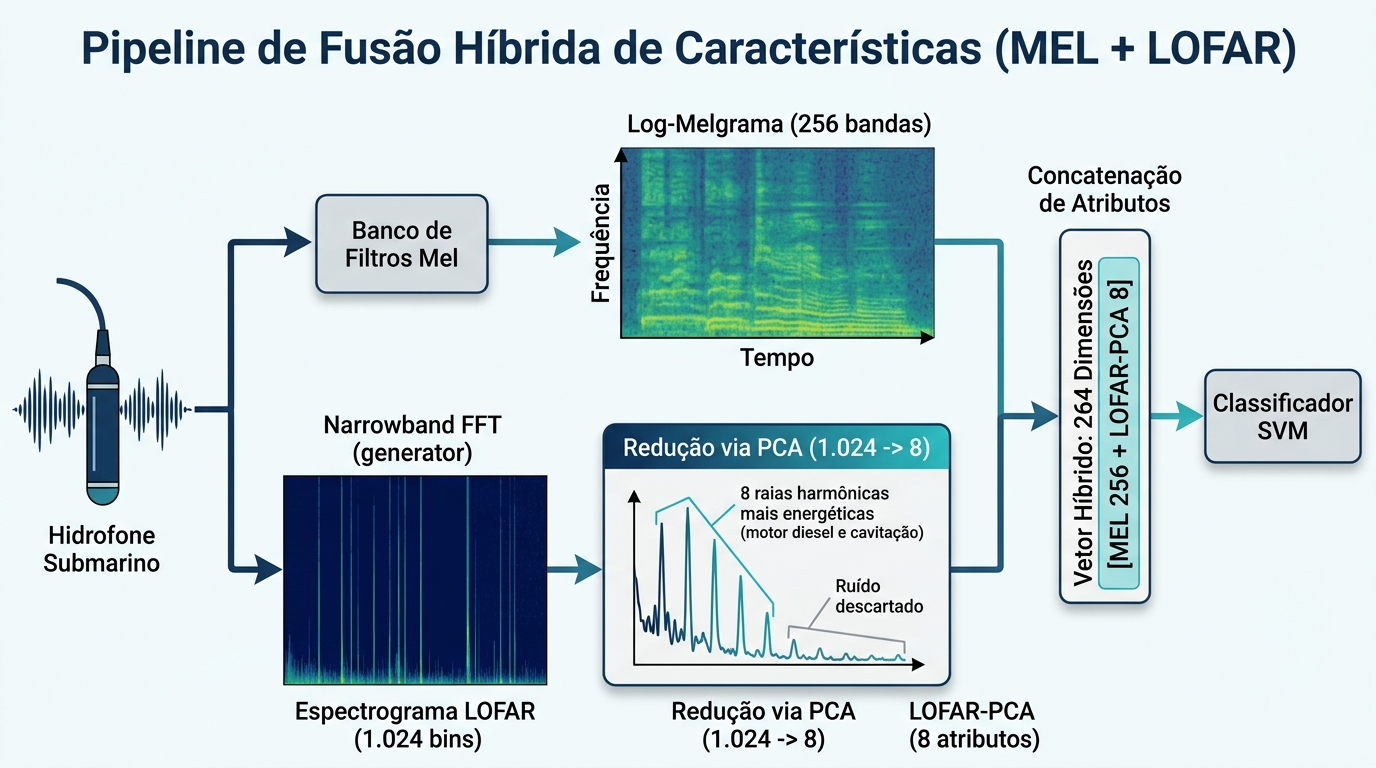
\includegraphics[width=0.83\textwidth,height=0.44\textheight,keepaspectratio]{imgs/fusao_hibrida_mel_lofar_pt.jpg}
    
    \vspace{0.02cm}
    \begin{columns}[t]
        \column{0.49\textwidth}
        \begin{block}{\small 1. Fus\~{a}o de Caracter\'{i}sticas (264-D)}
            \scriptsize
            \begin{itemize}
                \setlength{\itemsep}{2pt}
                \item \textbf{Vetor Combinado:} Concatena\c{c}\~{a}o direta de \textbf{MEL (256-D)} com \textbf{LOFAR-PCA (8-D)}.
                \item \textbf{Papel do PCA-8:} Comprime o LOFAR de 1.024 para as 8 componentes de maior vari\^{a}ncia (efeito sobre o sobreajuste n\~{a}o testado).
            \end{itemize}
        \end{block}
        
        \column{0.49\textwidth}
        \begin{block}{\small 2. Roteamento em Cascata}
            \scriptsize
            \begin{itemize}
                \setlength{\itemsep}{2pt}
                \item \textbf{Acionamento:} s\'{o} se o modelo base prediz \textbf{LARGE} (janela a janela).
                \item \textbf{Resgate:} se n\~{a}o confirmar LARGE, vira \textbf{SMALL}: 293 SMALL resgatados de LARGE (10 folds), mas 146 MEDIUM corretos viraram SMALL.
            \end{itemize}
        \end{block}
    \end{columns}
\end{frame}

%--- SLIDE: Matrizes de Confusão em Porcentagem ---
\begin{frame}{Impacto da Cascata: Matrizes de Confus\~{a}o (\%)}
    \centering
    \scriptsize
    \textit{Linhas = classe real \ | \ Colunas = predi\c{c}\~{a}o \ | \ Avalia\c{c}\~{a}o por \'{a}udio ($5\times2$cv, 10 folds acumulados; especialista SL retreinado)}

    \vspace{0.1cm}
    \begin{columns}[T]
        \column{0.49\textwidth}
        \centering \textbf{SVM LOFAR 6000 (Base)} \\[0.05cm]
        \resizebox{0.98\columnwidth}{!}{%
        \begin{tabular}{r|cccc|c}
             & \textbf{S} & \textbf{M} & \textbf{L} & \textbf{BG} & \textbf{Rec.} \\ \hline
            \textbf{SMALL}  & \calo{38,1} & 22,8        & \calo{28,7} & 10,4 & $38,1\%$ \\
            \textbf{MEDIUM} & 17,6        & \cahi{60,4} & 17,2        &  4,8 & $60,4\%$ \\
            \textbf{LARGE}  &  9,2        & 10,9        & \cahi{76,3} &  3,6 & $76,3\%$ \\
            \textbf{BG}     &  6,1        &  2,8        &  4,1        & \cahi{87,0} & $87,0\%$ \\ \hline
            \textbf{Prec.}  & 56,7\%      & 57,5\%      & 66,9\%      & 71,9\% &
        \end{tabular}}
        \vspace{0.05cm}

        \scriptsize
        \textbf{ACC micro $63,6\%$ | bal. $65,5\%$ | SP $63,8\%$}

        \column{0.49\textwidth}
        \centering \textbf{Cascata LOFAR 6000 + SL (Proposta)} \\[0.05cm]
        \resizebox{0.98\columnwidth}{!}{%
        \begin{tabular}{r|cccc|c}
             & \textbf{S} & \textbf{M} & \textbf{L} & \textbf{BG} & \textbf{Rec.} \\ \hline
            \textbf{SMALL}  & \cahi{63,7} & 15,7        & \cahi{11,5} &  9,1 & $\mathbf{63,7\%}$ \\
            \textbf{MEDIUM} & 30,3        & \camd{57,7} &  7,9        &  4,2 & $57,7\%$ \\
            \textbf{LARGE}  & 23,5        &  9,4        & \camd{63,5} &  3,6 & $63,5\%$ \\
            \textbf{BG}     &  9,9        &  2,0        &  2,3        & \cahi{85,7} & $85,7\%$ \\ \hline
            \textbf{Prec.}  & 51,9\%      & 63,1\%      & \textbf{79,8\%} & 73,6\% &
        \end{tabular}}
        \vspace{0.05cm}

        \scriptsize
        \textbf{ACC micro $65,6\%$ | bal. $67,6\%$ | SP $67,2\%$}
    \end{columns}

    \vspace{0.15cm}
    \begin{block}{\small Principais Mudan\c{c}as:}
        \scriptsize
        \begin{itemize}
            \setlength{\itemsep}{1pt}
            \item \textbf{Recall SMALL:} $38,1\% \to \mathbf{63,7\%}$ (\textbf{+25,5 p.p.}) | Confus\~{a}o S$\to$L: $28,7\% \to \mathbf{11,5\%}$ | \textbf{Recall LARGE:} $76,3\% \to 63,5\%$ ($-12,8$ p.p.)
            \item \textbf{Precis\~{a}o LARGE:} $66,9\% \to \mathbf{79,8\%}$ (\textbf{+12,9 p.p.})
            \item \textbf{SP global:} $63,8\% \to \mathbf{67,2\%}$ (\textbf{+3,3 p.p.}; F-test $5\times2$cv $p=0,007$ vs. base) | \textbf{ACC micro:} $63,6\% \to 65,6\%$ (+2,0 p.p.)
        \end{itemize}
    \end{block}
\end{frame}

%--- SLIDE: Matrizes de Confusão com Valores Absolutos ---
\begin{frame}{Impacto da Cascata: Contagem Bruta de \'{A}udios}
    \centering
    \scriptsize
    \textit{N\'{u}mero absoluto de avalia\c{c}\~{o}es por \'{a}udio (10 folds acumulados, 6.390 testes no total)}

    \vspace{0.1cm}
    \begin{columns}[T]
        \column{0.49\textwidth}
        \centering \textbf{SVM LOFAR 6000 (Base)} \\[0.05cm]
        \resizebox{0.98\columnwidth}{!}{%
        \begin{tabular}{r|rrrr|r}
             & \textbf{S} & \textbf{M} & \textbf{L} & \textbf{BG} & \textbf{Total} \\ \hline
            \textbf{SMALL}  & \calo{679}  & 405  & \calo{511}  & 185 & 1.780 \\
            \textbf{MEDIUM} & 262         & \cahi{900}  & 257         &  71 & 1.490 \\
            \textbf{LARGE}  & 197         & 233         & \cahi{1.633} &  77 & 2.140 \\
            \textbf{BG}     &  60         &  27         &  40         & \cahi{853} &   980 \\
        \end{tabular}}
        \vspace{0.05cm}

        \scriptsize
        Corretos: 4.065/6.390 \\
        \textbf{ACC micro: $63,6\%$ | SP: $63,8\%$}

        \column{0.49\textwidth}
        \centering \textbf{Cascata LOFAR 6000 + SL (Proposta)} \\[0.05cm]
        \resizebox{0.98\columnwidth}{!}{%
        \begin{tabular}{r|rrrr|r}
             & \textbf{S} & \textbf{M} & \textbf{L} & \textbf{BG} & \textbf{Total} \\ \hline
            \textbf{SMALL}  & \cahi{1.133} & 280  & \cahi{205}  & 162 & 1.780 \\
            \textbf{MEDIUM} & 452          & \camd{859}  & 117         &  62 & 1.490 \\
            \textbf{LARGE}  & 502          & 202         & \camd{1.359} &  77 & 2.140 \\
            \textbf{BG}     &  97          &  20         &  23         & \cahi{840} &   980 \\
        \end{tabular}}
        \vspace{0.05cm}

        \scriptsize
        Corretos: \textbf{4.191}/6.390 (\textbf{+126}) \\
        \textbf{ACC micro: $65,6\%$ | SP: $67,2\%$}
    \end{columns}

    \vspace{0.15cm}
    \begin{block}{\small Ganhos e Perdas em N\'{u}meros Absolutos:}
        \scriptsize
        \begin{itemize}
            \setlength{\itemsep}{1pt}
            \item \textbf{Resgate de SMALL:} De 679 para \textbf{1.133} corretos (\textbf{+454}), com confus\~{a}o S$\to$L caindo de 511 para \textbf{205}.
            \item \textbf{LARGE:} De 1.633 para 1.359 corretos ($\mathbf{-274}$); L$\to$S sobe de 197 para 502. \textbf{MEDIUM:} De 900 para 859 ($-41$) --- efeito colateral da reclassifica\c{c}\~{a}o janela a janela. \textbf{BG:} $-13$.
            \item \textbf{Saldo total:} \textbf{+126} avalia\c{c}\~{o}es corretas (de 6.390). Cada \'{a}udio aparece em m\'{e}dia em 3,75 folds de teste; as contagens n\~{a}o s\~{a}o \'{a}udios \'{u}nicos.
        \end{itemize}
    \end{block}
\end{frame}

\begin{frame}{Efeito Colateral: Impacto do Especialista SL sobre MEDIUM e LARGE}
    \footnotesize
    Embora o Especialista SL atue \textbf{exclusivamente} na distin\c{c}\~{a}o SMALL vs. LARGE, ele gerou efeitos colaterais em MEDIUM e, sobretudo, em LARGE:

    \vspace{0.15cm}
    \begin{table}[h]
    \centering
    \resizebox{0.92\textwidth}{!}{%
    \begin{tabular}{l|cccc|c}
    \toprule
    \textbf{Recall por Classe (m\'{e}dia 10 folds)} & \textbf{SMALL} & \textbf{MEDIUM} & \textbf{LARGE} & \textbf{BG} & \textbf{\'{I}ndice SP} \\
    \midrule
    SVM LOFAR 6000 (Base) & \calo{$38,15\%$} & \cahi{$60,40\%$} & \cahi{$76,31\%$} & \cahi{$87,04\%$} & $63,83 \pm 1,91\%$ \\
    Cascata + SL (Proposta) & \cahi{$63,65\%$} & \camd{$57,65\%$} & \camd{$63,50\%$} & \cahi{$85,71\%$} & $\mathbf{67,16 \pm 1,82\%}$ \\
    \midrule
    \textbf{Varia\c{c}\~{a}o} & \textbf{+25,51 p.p.} & $-2,75$ p.p. & $-12,80$ p.p. & $-1,33$ p.p. & \textbf{+3,33 p.p.} ($p=0,007$) \\
    \bottomrule
    \end{tabular}%
    }
    \end{table}

    \vspace{0.1cm}
    \begin{columns}[t]
        \column{0.55\textwidth}
        \begin{alertblock}{\small Por que MEDIUM caiu se o SL n\~{a}o toca nele?}
            \scriptsize
            A cascata atua \textbf{janela a janela} ($0,512\text{ s}$). Em um navio MEDIUM, parte das janelas \'{e} classificada como LARGE pelo multiclasse. O Especialista SL converte essas janelas para SMALL, inflando os votos de SMALL na \textbf{vota\c{c}\~{a}o majorit\'{a}ria} do \'{a}udio e invertendo o resultado final de MEDIUM para SMALL (146 avalia\c{c}\~{o}es MEDIUM corretas passaram a SMALL). Pelo mesmo mecanismo, 502 avalia\c{c}\~{o}es LARGE terminam como SMALL (eram 197).
        \end{alertblock}

        \column{0.44\textwidth}
        \begin{block}{\small Por que o SP subiu mesmo assim?}
            \scriptsize
            O \'{I}ndice SP combina m\'{e}dia aritm\'{e}tica e \textbf{m\'{e}dia geom\'{e}trica} dos recalls, que penaliza o menor termo. Como SMALL era o gargalo ($38,15\%$), o salto para $63,65\%$ compensou as perdas em MEDIUM ($-2,75$) e LARGE ($-12,80$ p.p.).
        \end{block}
    \end{columns}
\end{frame}

\begin{frame}{Robustez ao CPA: Desempenho da Cascata nos Regimes Ac\'{u}sticos}
    \footnotesize
    Desempenho por cole\c{c}\~{a}o do \'{a}udio de teste (modelos de 4 classes; re-execu\c{c}\~{o}es locais, $5\times2$cv):

    \begin{table}[h]
    \centering
    \resizebox{0.88\textwidth}{!}{%
    \begin{tabular}{l|cc|cc|c}
    \toprule
    \textbf{Modelo} & \textbf{Near CPA (A)} & \textbf{Far CPA (C)} & \textbf{CPA IN (A+C)} & \textbf{CPA OUT (B+D)} & \textbf{Geral ($5\times2$cv)} \\
    \midrule
    MLP LOFAR \textit{(local)}        & \cahi{$67,0\% \ (68,1\%)$} & $59,7\% \ (61,2\%)$ & $64,2\% \ (65,3\%)$ & \cahi{$52,3\% \ (52,6\%)$} & $66,2\% \ (67,2\%)$ \\
    MLP MEL \textit{(local)}          & $62,6\% \ (64,0\%)$ & $61,0\% \ (62,6\%)$ & $62,3\% \ (63,6\%)$ & $50,1\% \ (50,6\%)$ & $64,7\% \ (65,7\%)$ \\
    CNN MEL \textit{(local)}          & $60,2\% \ (61,9\%)$ & $58,4\% \ (60,0\%)$ & $59,9\% \ (61,3\%)$ & $48,3\% \ (48,9\%)$ & $63,8\% \ (65,0\%)$ \\
    MLP H\'{i}brido \textit{(MEL+LOFAR-PCA64)} & $63,1\% \ (64,6\%)$ & $63,0\% \ (64,0\%)$ & $63,6\% \ (64,6\%)$ & $52,2\% \ (52,5\%)$ & $66,1\% \ (66,9\%)$ \\
    SVM LOFAR 6000 \textit{(Base)}    & $62,3\% \ (64,2\%)$ & $56,8\% \ (59,0\%)$ & $60,4\% \ (62,2\%)$ & $50,2\% \ (50,8\%)$ & $63,8\% \ (65,5\%)$ \\
    \midrule
    \textbf{Cascata LOFAR + SL} (janela) & $65,3\% \ (65,8\%)$ & \cahi{$\mathbf{64,4\% \ (65,4\%)}$} & \cahi{$\mathbf{65,6\% \ (66,0\%)}$} & $51,7\% \ (52,6\%)$ & \cahi{$\mathbf{67,2\% \ (67,6\%)}$} \\
    Cascata LOFAR + SL (arquivo)      & $64,6\% \ (65,3\%)$ & $61,9\% \ (63,2\%)$ & $64,0\% \ (64,6\%)$ & $51,0\% \ (51,4\%)$ & $66,0\% \ (66,8\%)$ \\
    \midrule
    \textit{$p$ cascata (janela) vs. MLP LOFAR} & $0,71$ & $0,056$ & $0,65$ & $0,40$ & $0,56$ \\
    \bottomrule
    \end{tabular}%
    }
    \end{table}
    \vspace{-0.25cm}
    \centering \tiny \textit{Formato: SP \% (Acur\'{a}cia Balanceada \%). Cole\c{c}\~{o}es A--D t\^{e}m s\'{o} navios (SP sobre 3 classes); BACKGROUND (E) entra s\'{o} em ``Geral''.}

    \begin{block}{\small An\'{a}lise de Robustez Espectral:}
        \scriptsize
        \begin{itemize}
            \setlength{\itemsep}{1pt}
            \item \textbf{Melhora no Far CPA (C):} o SP subiu de $56,8\%$ (base) para $\mathbf{64,4\%}$ ($+7,6$ p.p., $p=0,003$). Frente ao MLP LOFAR ($59,7\%$) a diferen\c{c}a ($+4,7$ p.p.) n\~{a}o \'{e} significativa ($p=0,056$), e o MLP H\'{i}brido chega a $63,0\%$ ($p=0,39$).
            \item \textbf{Near CPA (A):} a cascata ($65,3\%$) fica \textbf{abaixo} em m\'{e}dia do MLP LOFAR ($67,0\%$; $p=0,71$).
            \item \textbf{CPA OUT (B+D):} todos os modelos caem para $48$--$52\%$; a cascata ($51,7\%$) \'{e} equivalente ao MLP LOFAR ($52,3\%$; $p=0,40$).
        \end{itemize}
    \end{block}
\end{frame}

\begin{frame}{Ranking Geral Consolidado de Todos os Modelos}
    \footnotesize
    Ordem decrescente da m\'{e}dia do \textbf{\'{I}ndice SP} ($5\times2$cv por \'{a}udio); $p$ = F-test $5\times2$cv vs. MLP LOFAR local:

    \begin{table}[h]
    \centering
    \resizebox{0.90\textwidth}{!}{%
    \begin{tabular}{c|llccc|l}
    \toprule
    \textbf{Pos.} & \textbf{Modelo / Arquitetura} & \textbf{Espectro} & \textbf{\'{I}ndice SP (\%)} & \textbf{Acur. Bal. (\%)} & \textbf{$p$} & \textbf{Fonte / Destaque} \\
    \midrule
    1\textsuperscript{o} & \textbf{SVM em Cascata por janela (LOFAR 6000 + SL)} & H\'{i}brido & \cahi{$\mathbf{67,16 \pm 1,82}$} & $67,63 \pm 1,87$ & $0,56$ & Local; $p=0,007$ vs. SVM base \\
    2\textsuperscript{o} & \textbf{MLP [32, 16] LOFAR} & LOFAR & \cart{$\mathbf{66,51 \pm 1,39}$} & \cart{$\mathbf{67,48 \pm 1,24}$} & --- & Artigo (Tabela 7): benchmark \\
    3\textsuperscript{o} & MLP [32, 16] LOFAR & LOFAR & $66,24 \pm 1,78$ & $67,22 \pm 1,65$ & ref. & Local (re-execu\c{c}\~{a}o) \\
    4\textsuperscript{o} & MLP H\'{i}brido (MEL + LOFAR-PCA64) & H\'{i}brido & $66,13 \pm 1,09$ & $66,92 \pm 1,06$ & $0,67$ & Local \\
    5\textsuperscript{o} & CNN Convolucional LOFAR & LOFAR & $66,05 \pm 1,90$ & $67,02 \pm 1,78$ & --- & Artigo (Tabela 7) \\
    6\textsuperscript{o} & SVM em Cascata por arquivo (LOFAR 6000 + SL) & H\'{i}brido & $66,00 \pm 1,90$ & $66,77 \pm 1,92$ & $0,37$ & Local; $p=0,030$ vs. SVM base \\
    7\textsuperscript{o} & MLP [32, 16] MEL & MEL-256 & $64,74 \pm 2,05$ & $65,73 \pm 1,90$ & $0,65$ & Local (artigo: $63,38$) \\
    8\textsuperscript{o} & SVM Nystr\"{o}m LOFAR ($m=6000$) & LOFAR & $63,83 \pm 1,91$ & $65,47 \pm 1,77$ & $0,15$ & Local; melhor SVM isolado \\
    9\textsuperscript{o} & CNN Convolucional MEL & MEL-256 & $63,80 \pm 2,23$ & $65,01 \pm 2,05$ & $0,22$ & Local (artigo: $63,52$) \\
    10\textsuperscript{o} & SVM Nystr\"{o}m MEL ($m=4000$) & MEL-256 & $63,78 \pm 1,14$ & $64,56 \pm 1,18$ & $0,27$ & Local; menor desvio \\
    11\textsuperscript{o} & Random Forest (RF) MEL & MEL-256 & $62,22 \pm 1,86$ & $62,64 \pm 1,84$ & --- & Artigo (Tabela 7) \\
    12\textsuperscript{o} & Random Forest (RF) LOFAR & LOFAR & $56,92 \pm 1,69$ & $58,87 \pm 1,68$ & --- & Artigo (Tabela 7) \\
    \bottomrule
    \end{tabular}%
    }
    \end{table}

    \vspace{0.1cm}
    \begin{block}{\small Conclus\~{o}es Finais do Benchmark:}
        \scriptsize
        \begin{itemize}
            \setlength{\itemsep}{1pt}
            \item \textbf{Sem supera\c{c}\~{a}o estat\'{i}stica do benchmark:} a melhor cascata ($67,16 \pm 1,82\%$) \'{e} \textbf{equivalente} ao MLP LOFAR local ($66,24\%$; $p=0,56$) e fica $+0,65$ p.p. acima do MLP LOFAR do artigo ($66,51 \pm 1,39\%$), dentro do desvio. Nenhum modelo local difere significativamente do MLP LOFAR.
            \item \textbf{Ganho real sobre o pr\'{o}prio SVM:} a cascata melhora o SVM LOFAR base ($63,83 \to 67,16\%$, $p=0,007$) ao resgatar SMALL ($38,15 \to 63,65\%$), \`{a} custa de LARGE ($76,31 \to 63,50\%$).
        \end{itemize}
    \end{block}
\end{frame}

%===========================================
% SEÇÃO 11: DISCUSSÃO E PRÓXIMOS PASSOS
%===========================================
\section{Discuss\~{a}o e Pr\'{o}ximos Passos}

\begin{frame}{Discuss\~{a}o: D\'{u}vidas e Pr\'{o}ximos Passos da Pesquisa}
    \footnotesize
    Pontos abertos para discuss\~{a}o e direcionamento das pr\'{o}ximas etapas:

    \vspace{0.02cm}
    \begin{columns}[t]
        \column{0.49\textwidth}
        \begin{block}{\small 1. Meta de Desempenho e Artigo}
            \scriptsize
            \begin{itemize}
                \setlength{\itemsep}{0pt}
                \item Devemos tentar sempre melhorar o SP ou temos outros objetivos? 
                \item Qual o patamar de SP almejado? (hoje $\mathbf{67,2\%}$, equivalente ao MLP LOFAR)
                \item Resultados sustentam novo artigo? (sem supera\c{c}\~{a}o estat\'{i}stica do artigo; ganho significativo s\'{o} sobre o SVM base).
            \end{itemize}
        \end{block}

        \vspace{0.02cm}
        \begin{block}{\small 2. Novos Formatos de Entrada}
            \scriptsize
            \begin{itemize}
                \setlength{\itemsep}{0pt}
                \item Vale a pena estudar entradas al\'{e}m de LOFAR e MEL?
                \item \textbf{DEMON}: \textit{Demodulation of Envelope}
                \item \textbf{MFCC}: \textit{Mel-Frequency Cepstral Coefficients}
            \end{itemize}
        \end{block}

        \column{0.49\textwidth}
        \begin{block}{\small 3. Extra\c{c}\~{a}o e Expans\~{a}o de Dados}
            \scriptsize
            \begin{itemize}
                \setlength{\itemsep}{0pt}
                \item Extrair novos recortes dados do IARA?
                \item Avaliar \textit{Data Augmentation} ac\'{u}stico?
            \end{itemize}
        \end{block}

        \vspace{0.02cm}
        \begin{block}{\small 4. Avalia\c{c}\~{a}o de Novos Modelos}
            \scriptsize
            \begin{itemize}
                \setlength{\itemsep}{0pt}
                \item Quais modelos podemos explorar?  \textit{Gated Recurrent Unit} (GRU) ? \textit{Bi-GRU}? \textit{LSTM}? 
            \end{itemize}
        \end{block}
    \end{columns}
\end{frame}

%===========================================
% SLIDE FINAL
%===========================================
\begin{frame}
    \centering
    \Huge Obrigado!
    
    \vspace{0.5cm}
    \large
    
    
    \vspace{0.3cm}
    \normalsize
    Evandro Rocha\\
    UFRJ / COPPE / PEE
\end{frame}

\end{document}
